\section{Post-Processing of runs}

After we have kicked off the autoreduction and generated individual processed runs of the data, we can begin the post-processing step. Here, we can do more involved data reduction where we combine multiple runs for better statistics and data quality and perform more advanced corrections if needed.

\subsection{Load Runs into Table}

Below is the \guicmd{Post-Processing} tab: 

\noindent\makebox[\textwidth]{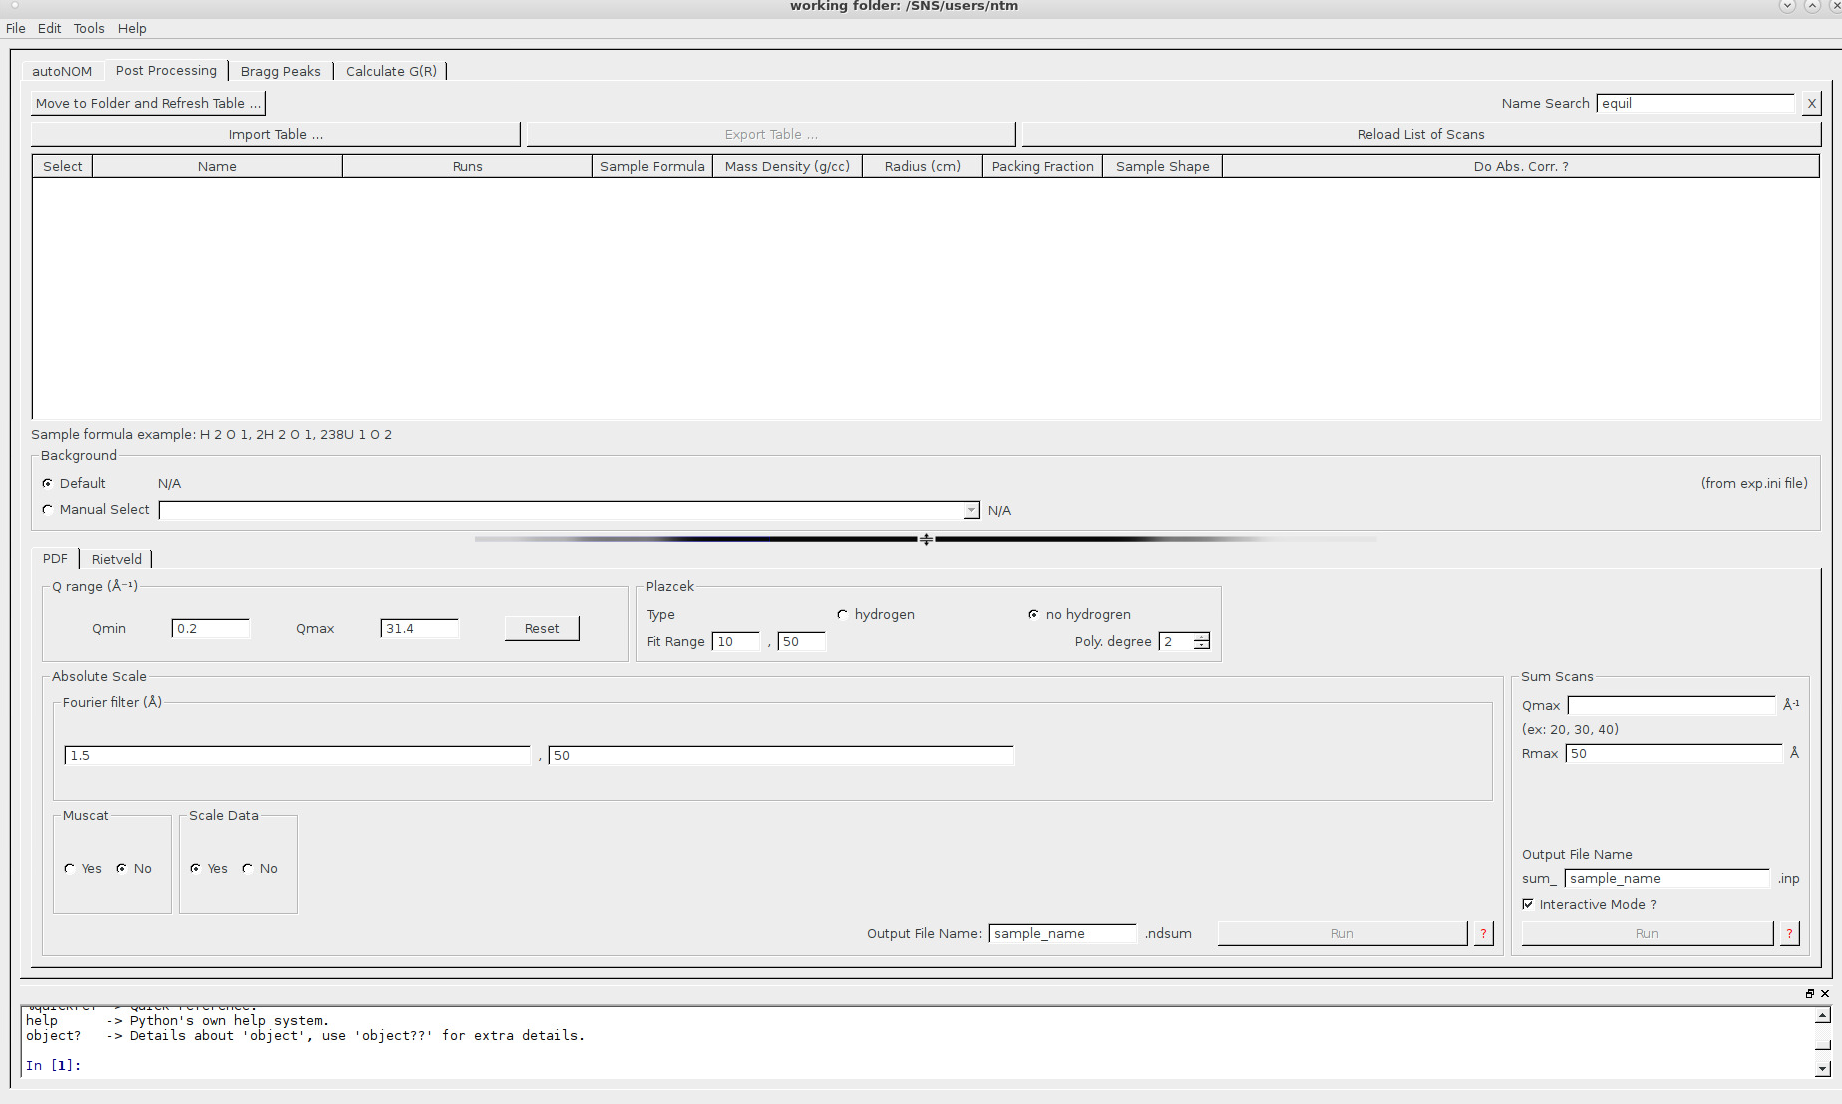
\includegraphics[width=0.9\paperwidth]{graphics/tab2/tab2.png}}

From here, we must first import our individual run information into the table. We do so by selecting the \guicmd{Move To Folder and Refresh Table...} button. We are presented with the following dialog box asking about the Dynamic Temperature. From the individual runs, the actual temperature of the experiment is appended to the title. We can remove this from the title to group runs together in a more effect way by checking the box. You can keep this temperature in the title to split up groups of runs to exclude ones that may not be actually at the correct temperature (due to equilibration from a temperature ramp taking longer than expected) by un-checking the box. Make your selection and press the \guicmd{Okay} button:

\noindent\makebox[\textwidth]{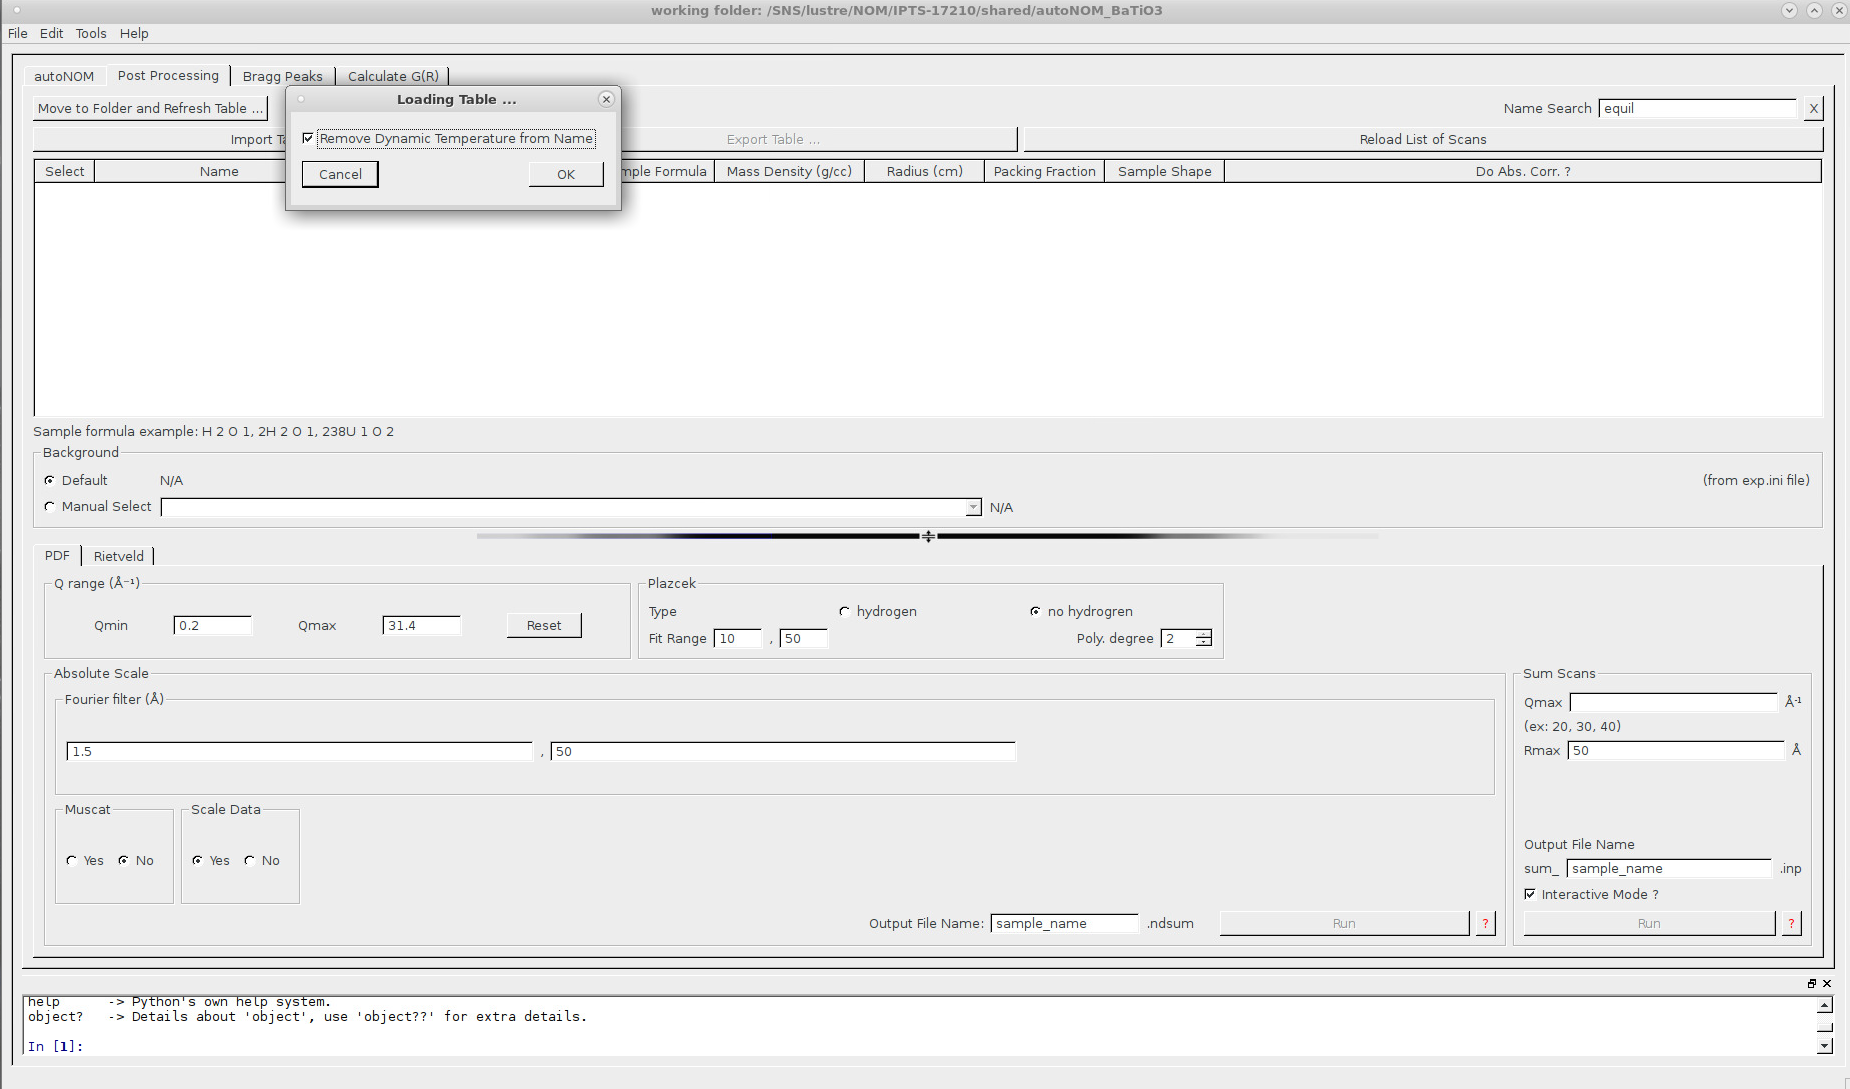
\includegraphics[width=0.9\paperwidth]{graphics/tab2/tab2_moveToFolderAndRefreshTable_removeDynamicTemperature.png}}

Next, the file dialog box will display to choose the directory where the List of Scans file is located that we will import. There are actually two versions of the file: a space-separated version (\fileio{los.txt}) and a comma-separated version (\fileio{los.csv}). In ADDIE, we read from the comma-separated version, the \fileio{los.csv} file. Navigate to the correct autoNOM directory like below and select the \guicmd{Choose} button.

\noindent\makebox[\textwidth]{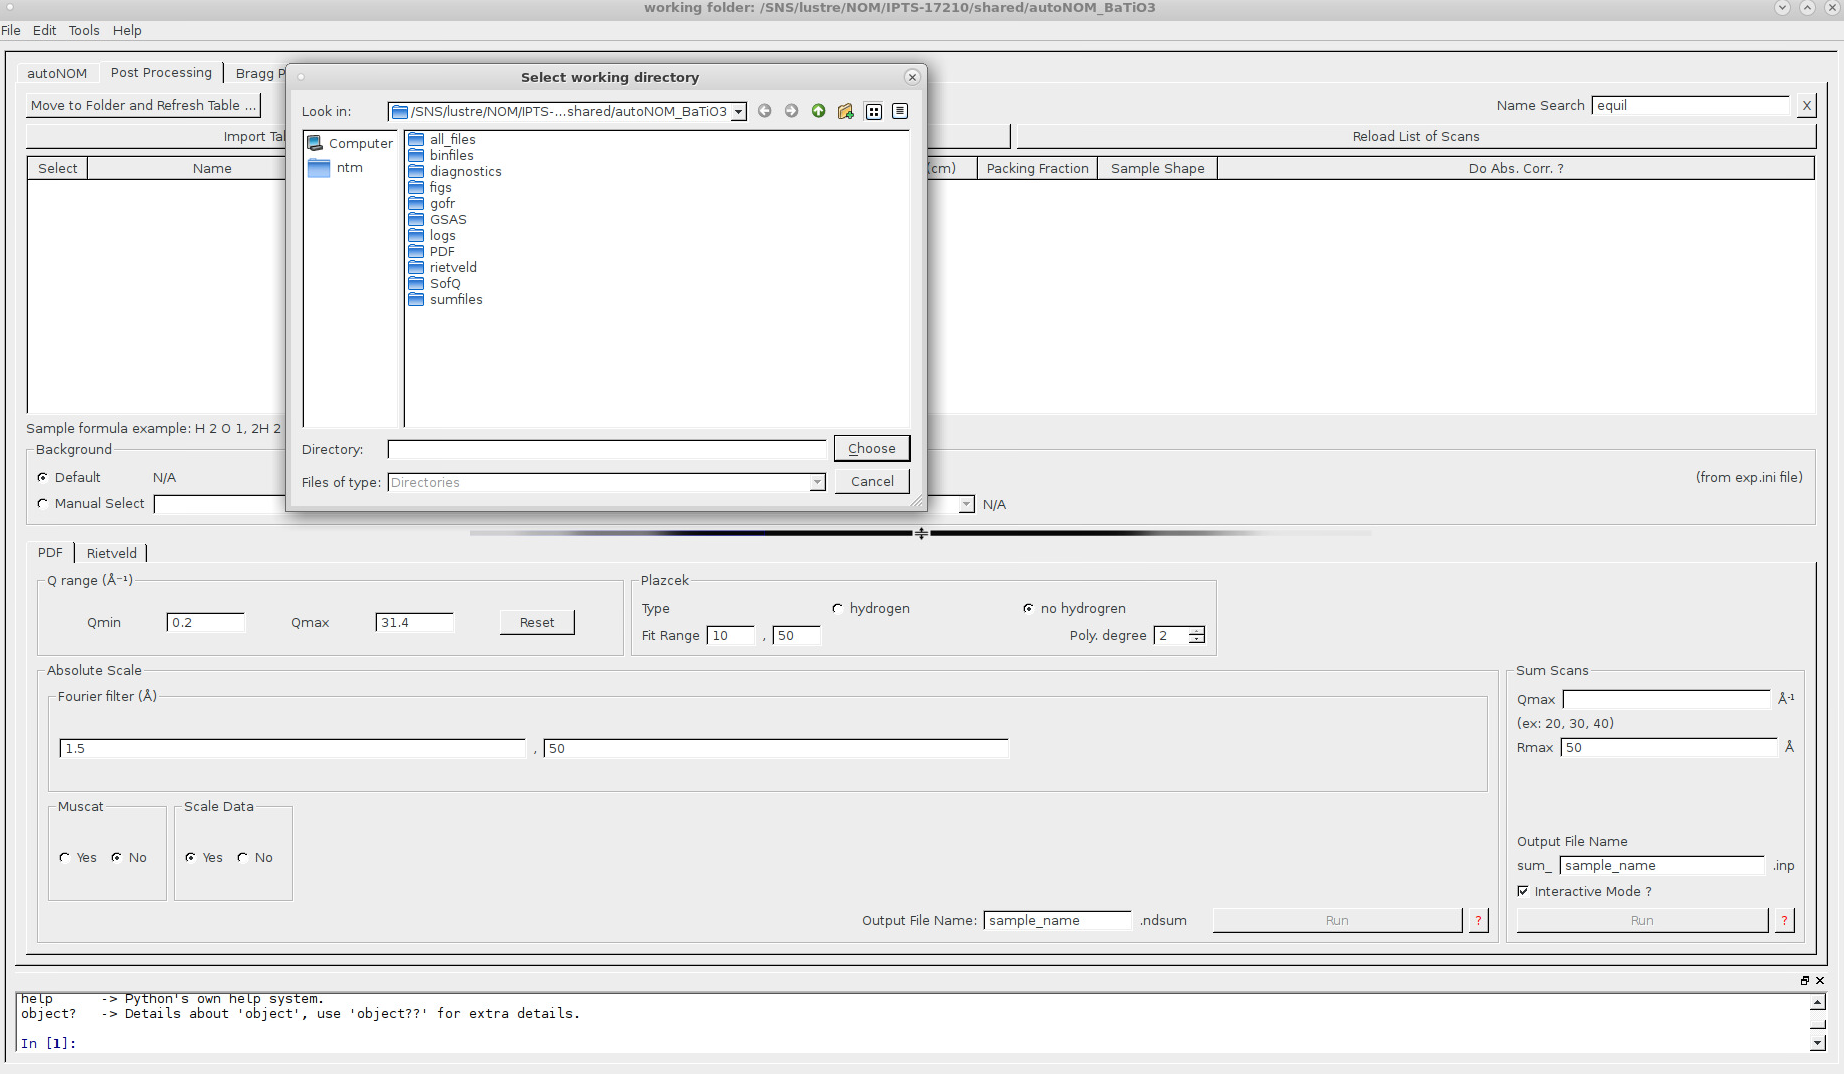
\includegraphics[width=0.9\paperwidth]{graphics/tab2/tab2_moveToFolderAndRefreshTable.png}}

Now, the table should be populated with your experiment runs with the individual runs grouped based on similar sample runs. 

\noindent\makebox[\textwidth]{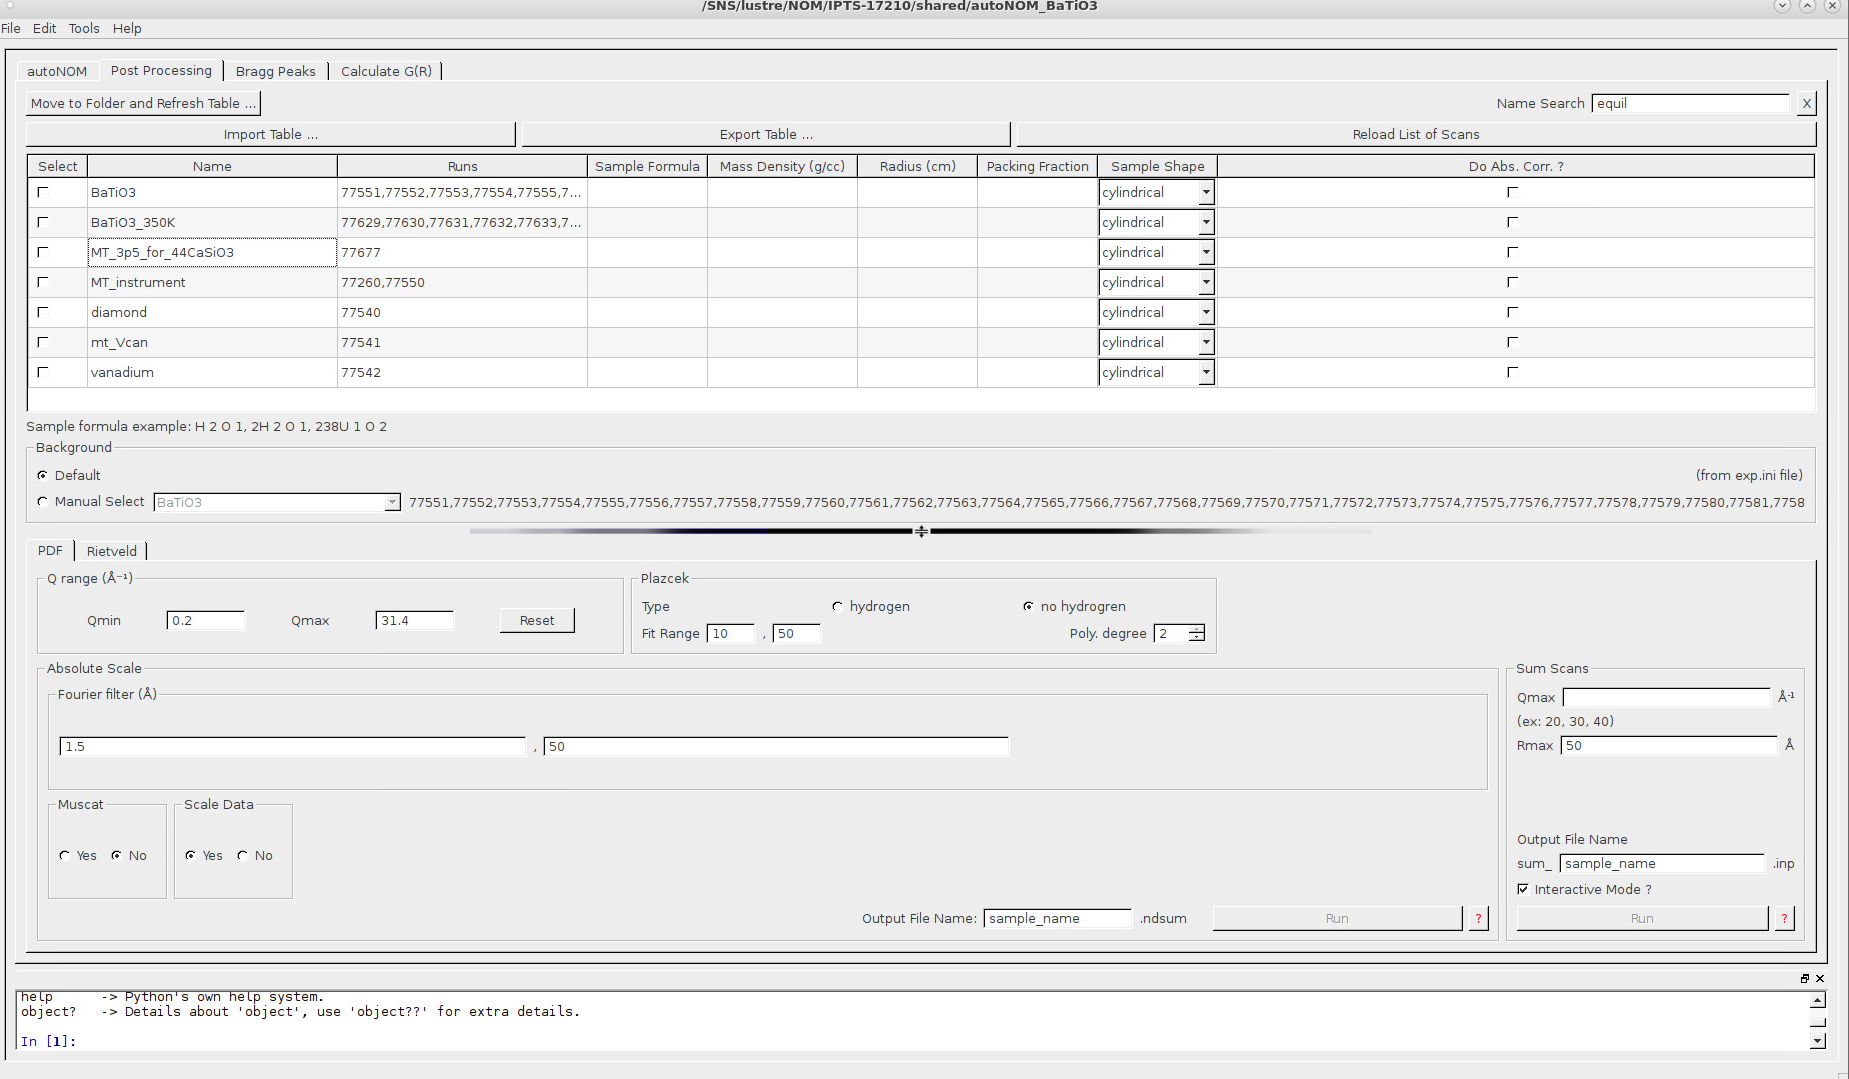
\includegraphics[width=0.9\paperwidth]{graphics/tab2/tab2_populatedTable.png}}

If you have trouble viewing the contents of the table based on your monitor (can be an issue with laptop displays), you can use the bar shown below to shrink the post-processing options below the table:

\noindent\makebox[\textwidth]{\includegraphics[width=0.5\paperwidth]{graphics/tab2/tab2_populatedTable_viewBar.png}}


\subsection{Selection of Runs from Table}

You can edit this table and export the changes using the \guicmd{Export Table...} command. Then, when you need to import those changes into the table for another session, you can use the \guicmd{Import Table...} to re-populate the table with the saved table. The \guicmd{Reload List of Scans...} button will refresh the table while an experiment is running and keep all the changes you have made. If you need to just start again, you can use the \guicmd{Refresh/Reset Table...} command from the right-click options described in more detail below. 

To edit any of the fields in the table, you can just double click and input any information you would like. This includes changing the name of the group or deleting runs for a given row. You can select multiple rows by holding the \textit{Ctrl} button for individual selections or holding down \textit{Shift} to chose a range of rows. You can right-click to get options for individual rows as well. 

\noindent\makebox[\textwidth]{\includegraphics[width=0.9\paperwidth]{graphics/tab2/tab2_populatedTable_rightClickOptions.png}}


These options are as follows:

\begin{itemize}

\item \guicmd{Undo}: Undo the last action in the table.
\item \guicmd{Redo}: Redo the last undone action in the table.
\item \guicmd{Copy}: Copy the selected contents of a field in a row.
\item \guicmd{Paste}: Paste copied contents in a field of a row.
\item \guicmd{Clear}: Clear the contents of a field in a row.
\item \guicmd{Check All}: Check all of the \guicmd{Select} boxes for all rows.
\item \guicmd{Unchecked All}: Uncheck all of the \guicmd{Select} boxes for all rows.
\item \guicmd{Inverse Selection}: Reverse the selection of the rows. Changes checked rows to unchecked rows and vice versa.
\item \guicmd{Insert Blank Row}: Insert an new, blank row.
\item \guicmd{Duplicate Row}: Duplicate an entire row in the table based on selection. 
\item \guicmd{Remove Row(s)}: Remove an entire row or rows based on selection.
\item \guicmd{Plot}: Plot the S(Q) for individual runs on the same plot (with an 0.2 offset on the y-axis). If the data has not finished processing or the S(Q) does not exists, it will not show up in the graph. An example is shown below:

\noindent\makebox[\textwidth]{\includegraphics[width=0.8\paperwidth]{graphics/tab2/tab2_populatedTable_rightClick_plot.png}}

\item \guicmd{Plot Diff (1st run)....}: Plot the difference in S(Q) for individual runs on the same plot (with an 0.2 offset on the y-axis) using the 1st listed run as the reference. If the data has not finished processing or the S(Q) does not exists, it will not show up in the graph. The run subtracted is the first run plotted and shows up as a horizontal line at 0 on the y-axis. An example is shown below:

\noindent\makebox[\textwidth]{\includegraphics[width=0.8\paperwidth]{graphics/tab2/tab2_populatedTable_rightClick_plotDiff1stRun.png}}

\item \guicmd{Plot Diff (Avg.)....}: Plot the difference in S(Q) for individual runs on the same plot (with an 0.2 offset on the y-axis) using the average of the runs as the reference. If the data has not finished processing or the S(Q) does not exists, it will not show up in the graph.  An example is shown below:


\noindent\makebox[\textwidth]{\includegraphics[width=0.8\paperwidth]{graphics/tab2/tab2_populatedTable_rightClick_plotDiffAvg.png}}

\item \guicmd{Refresh/Reset Table}: Reloads the table with the current List of Scans file (los.csv)

\item \guicmd{Clear Table...}: Removes all contents from the table.

\end{itemize}

You can add sample information into the table by editing the necessary fields. Below is an example for the barium titanate where the sample formula, mass density, radius of the sample can, and packing fraction have been input for the given row:

\noindent\makebox[\textwidth]{\includegraphics[width=0.9\paperwidth]{graphics/tab2/tab2_populatedTable_ndabs_sampleInfo.png}}\label{graphic_sampleInfo}

Once the table is in a good state, we are ready to begin post-processing for a given set of runs. We have already covered the options available for selecting runs based on the right-click options. You will need to have the \guicmd{Select} checkbox ticked for all rows that you want to use for post-processing. 

One tool that may also be of use is the \guicmd{Name Search} in the top right part of the tab. This allows you to select scans that match part of what you input into the field. Below, we show the BaTiO3 and BaTiO3\_350K rows that were selected based on a match with the "BaTi" input in the \guicmd{Name Search}.

\noindent\makebox[\textwidth]{\includegraphics[width=0.7\paperwidth]{graphics/tab2/tab2_populatedTable_nameSearch.png}}

This feature can help in selecting runs but also deleting unneeded runs. For example, if you have performed a temperature ramp and named the title of those runs "Ramp...", you can do a \guicmd{Name Search} to select those rows and then delete them via the right-click option. 

\subsection{Setting up and launching Post-Processing}

After the desired rows are selected, you can now set up the post-processing options. First, we begin by specifying the multiple background files to be subtracted from the data in the \guicmd{Background} section. These are typically your empty container runs (i.e. vanadium cans, capillaries, NMR tubes). The \guicmd{Default} will be the single empty container ruan that was used for the individual runs during the autoreduction. \guicmd{Manual select} will give you the option to select from one of the rows in the table. The run numbers for that row will be displayed beside this drop-down box. Any changes you make to the row in the table (change name, add/subtract run numbers) will be reflected for this drop-down and the runs displayed.

\noindent\makebox[\textwidth]{\includegraphics[width=0.7\paperwidth]{graphics/tab2/tab2_populatedTable_backgroundSelect.png}}

From here, there are two tabs to select from: 

\begin{itemize}

\item \guicmd{PDF}: Used for summing scans together and applying other corrections. Will produce Bragg profile and total scattering files. Uses autoNOM data reduction to perform the post-processing.

\item \guicmd{Rietveld}: Used for summing scans. Will produce Bragg profile files. Uses Mantid data reduction to perform the post-processing (specifically, the \snspowderreduction script).

\end{itemize}

\subsubsection{PDF Tab}

On the \guicmd{PDF} tab, we have two separate programs that can be launched: \guicmd{Sum Scans} and \guicmd{Absolute Scale}. The \guicmd{Q range}  and \guicmd{Plazcek} are sections that is common to both.

\begin{itemize}

\item \guicmd{Q range}: In this section, we can adjust $\text{Q}_min$ and $\text{Q}_max$, which are the minimum and maximum Q to use for the Fourier transform, respectively.

\item \guicmd{Plazcek}: In this section, we can select different hydrogen corrections and polynomial fits to the data and the range over which the correction is applied. 

The \guicmd{hyrdogen} button selects the correction that is described in Equation \ref{eq_nomad_Ipoly} under \textit{hyd=2} which is applied to Equation \ref{eq_nomad_SofQ}. 

The \guicmd{no hyrdogen} button selects the polynomial described in Equation \ref{eq_nomad_Ipoly} under \textit{hyd=0} which is applied to Equation \ref{eq_nomad_SofQ} with the degree of the polynomial chosen based on the value in the \guicmd{Poly. degree} field. 

The \guicmd{Fit Range} gives the limits in Q for these least-square fits for S(Q).

\item \guicmd{Sum Scans}: This is the driver for summing individual runs together. 

\guicmd{Qmax} allows for a list to use for the summed S(Q) datasets, where a simple truncation is performed. 

\guicmd{Rmax} specifies how far out in real-space the pair distribution function will be calculated. 

\guicmd{Output File Name} is just the name for the input file generated to run the \guicmd{Sum Scans} program externally.  

For \guicmd{Interacive Mode?}, when we run \guicmd{Sum Scans}, the external program produces diagnostic plots launched in x-terminals. If the \guicmd{Interacive Mode?} is selected, these plots will be displayed and the User must press \cmd{Enter} when finished looking at the plots. If the User does not wish to view the plots and let the program run "silently", uncheck the box before running. 

An example of these plots are shown below:

\end{itemize}

\noindent\makebox[\textwidth]{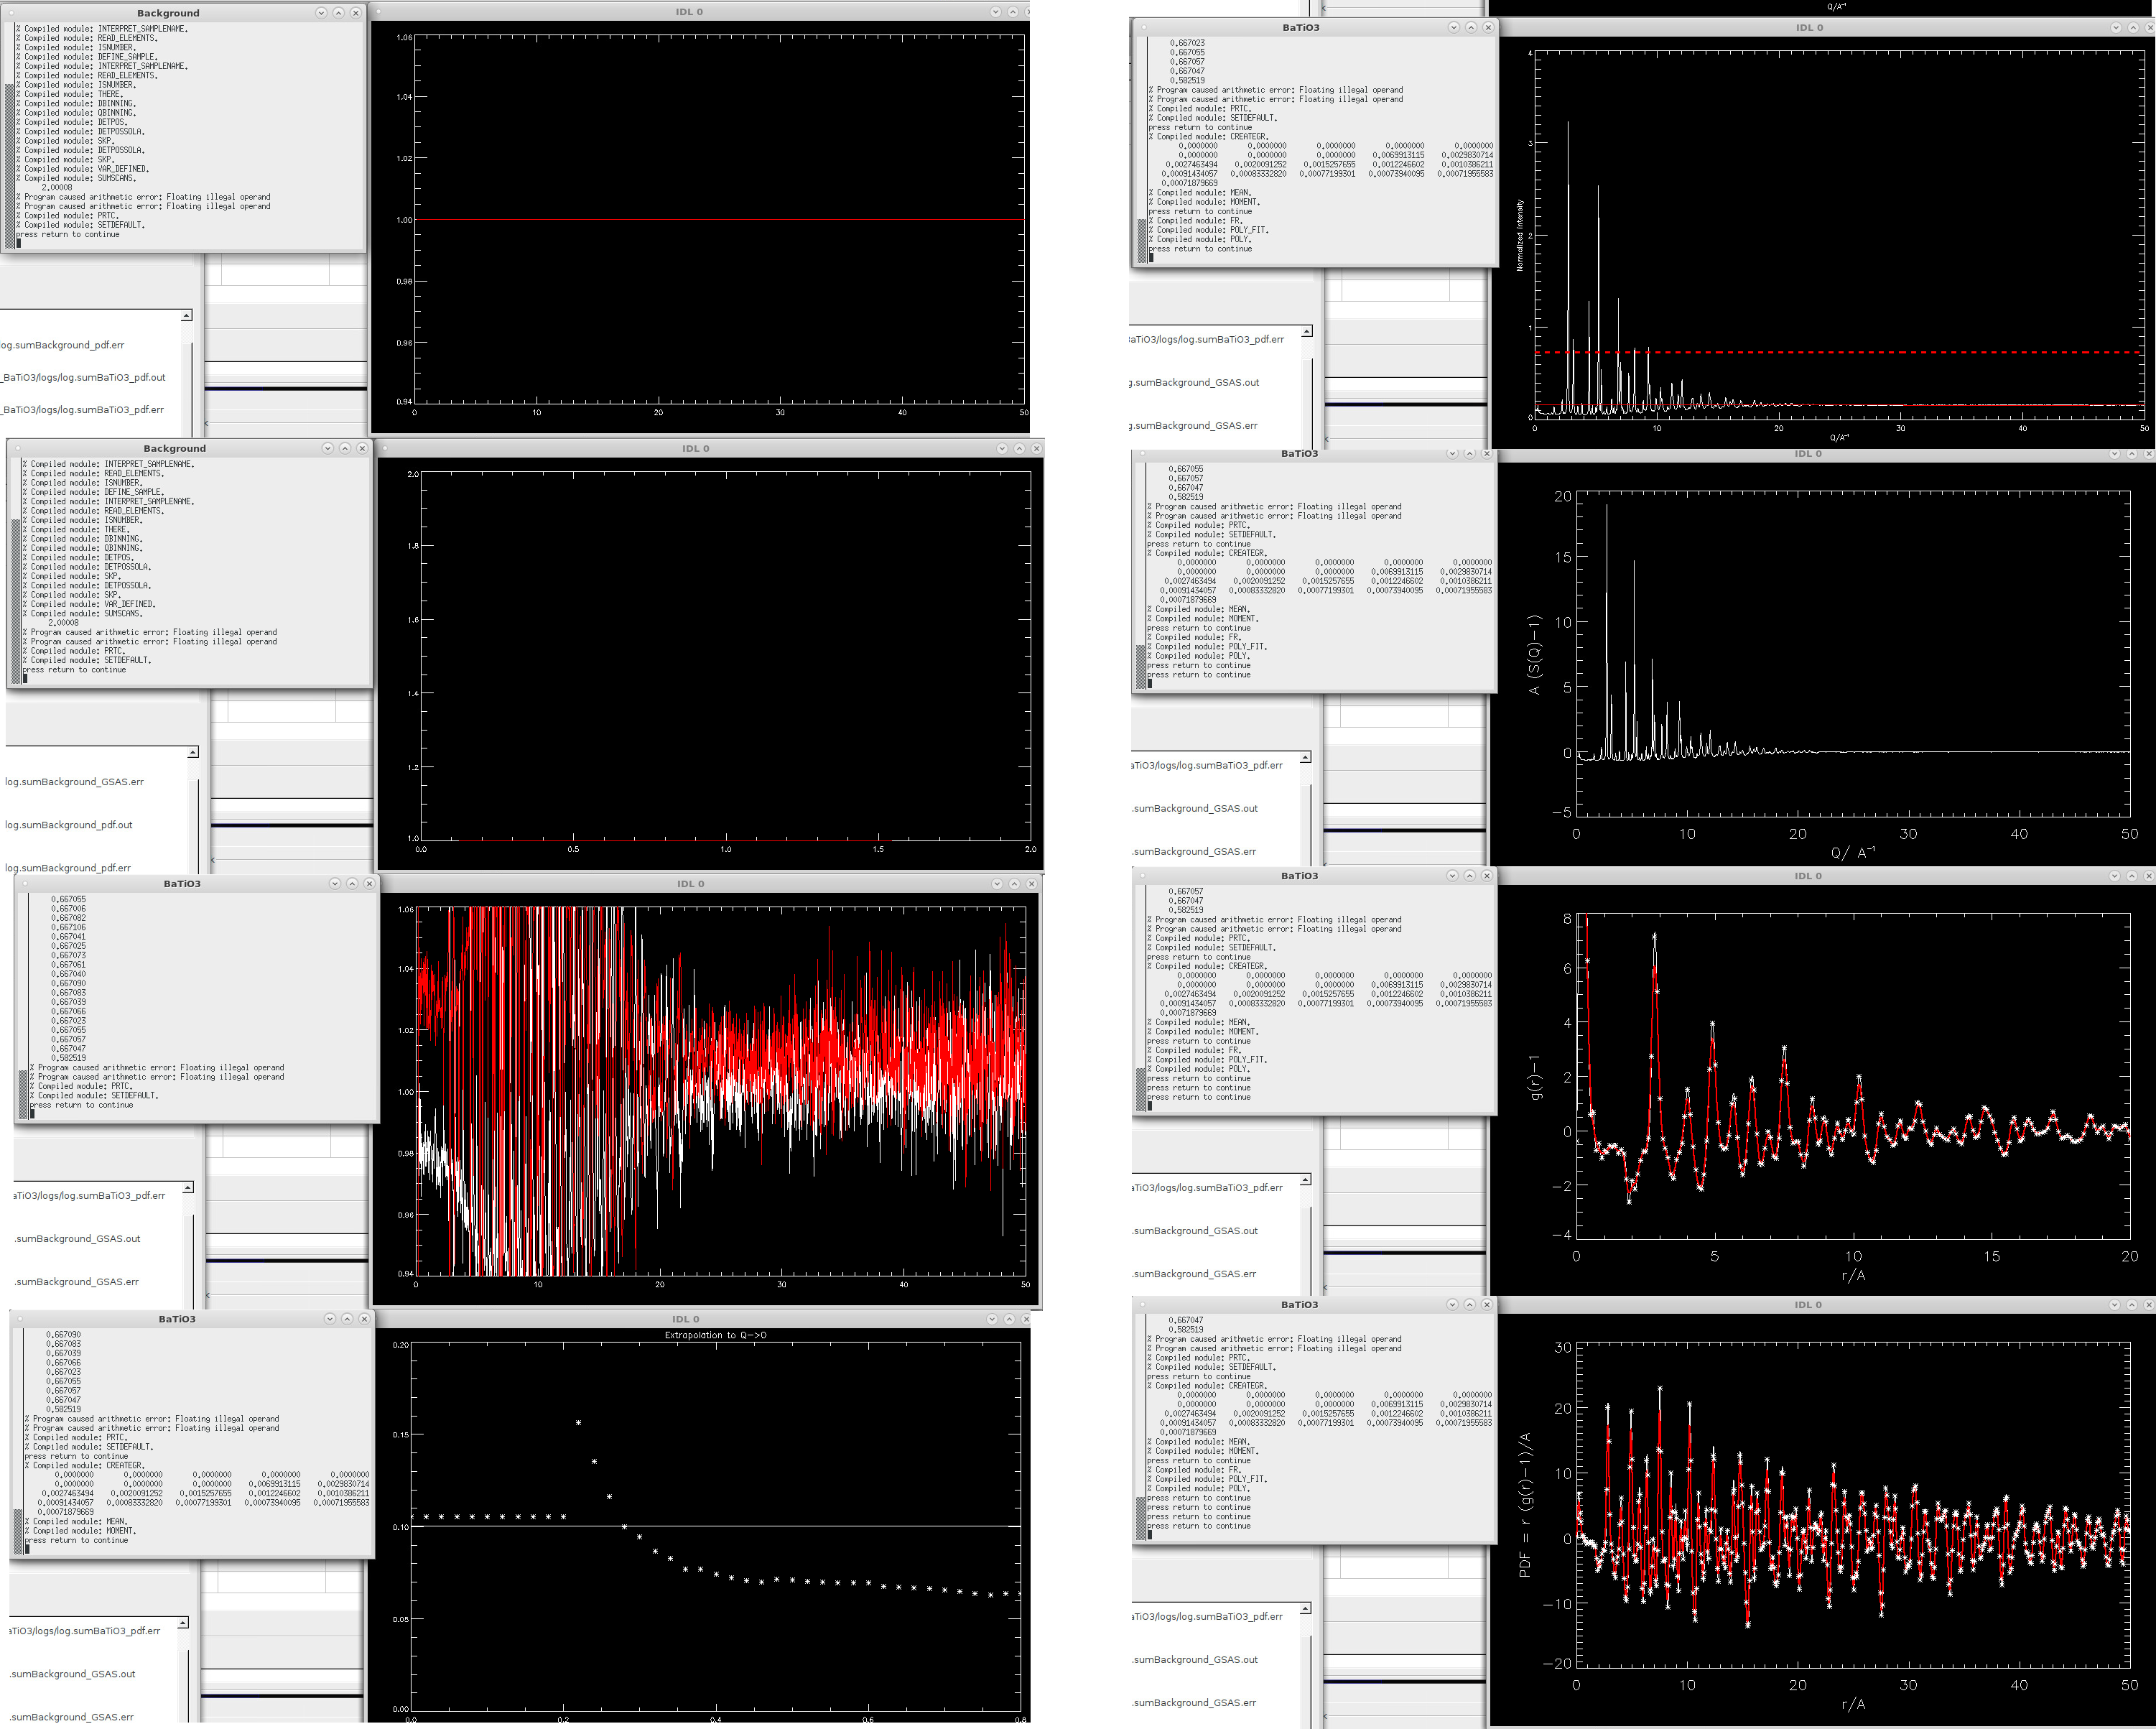
\includegraphics[width=0.9\paperwidth]{graphics/tab2/tab2_sumscans_plotsAll.png}}

\begin{itemize}

\item \guicmd{Absolute Scale} This is the driver for performing multiple scattering corrections and also to put the data on a absolute scale given the necessary information in the table. 

\guicmd{Fourier filter}: Specifies the real-space range for G(r) over which to apply a Fourier filter. This allows for "cropping" the real-space data by performing the reverse transform back to reciprocal space on the data outside the filter range, subtracts this reverse transform from the S(Q), and then transforms this S(Q) back to real-space G(r) with only the region specified by the Fourier filter.

\guicmd{Muscat}: Applies a multiple scattering absorption correction to the data based on both the sample material information and the geometry of the container specified in the table.

\guicmd{Scale Data}: Re-scales the data to a theoretical $\text{Q} \rightarrow \inf $ based on the sample density and packing fraction.


\end{itemize} 


\subsubsection{Rietveld Tab}

From the \guicmd{Rietveld} Tab, we can launch Mantid to also sum together runs and produce diffraction data. This mainly drives the \snspowderreduction algorithm found in Mantid used by other powder diffractometers at the SNS. Currently, the S(Q) and G(r) are not produced by this tab but is a work in progresss. The \guicmd{Rietveld} Tab is shown below:

\noindent\makebox[\textwidth]{\includegraphics[width=0.9\paperwidth]{graphics/tab2/tab2_populatedTable_rietveldTab.png}}

To launch the post-processing data reduction from this tab, you need to do the following:

\begin{itemize}

\item \guicmd{Browse Calibration...}: First, you need to select the appropriate calibration file to use. Press the \guicmd{Browse Calibration...} button to browse the calibration files available commonly shared to all NOMAD Users. Select one that is the most recent with the same sample environment that your experiment is using. You will see something similar to the selection below:

\noindent\makebox[\textwidth]{\includegraphics[width=0.9\paperwidth]{graphics/tab2/tab2_populatedTable_rietveldTab_calibration.png}}

\item \guicmd{Browse Characterization...}: Next, you must also select a characterization file for the instrument. Press the \guicmd{Browse Characterization...} button to browse the characterization files available commonly shared to all NOMAD Users. Select one that is the most recent. You will see something similar to the selection below:

\noindent\makebox[\textwidth]{\includegraphics[width=0.9\paperwidth]{graphics/tab2/tab2_populatedTable_rietveldTab_characterization.png}}

\item \guicmd{Number of Bins}: This defines the number of bins used along the x-axis. A negative value implies logarithmic binning, using the formula $x_{i+1} = x_i(1+|\Delta x_i|)$. More detail can be found \href{http://docs.mantidproject.org/nightly/algorithms/Rebin-v1.html}{here}.


\item \guicmd{Crop Wavelength}: Specify the minimum and maximum wavelength used to crop the TOF data. This data can also be found in the characterization file but can be overridden by the values specified here.

\item \guicmd{Vanadium Radius}: Specify the radius of the empty vanadium can container. This is used for applying the multiple scattering absorption correction.

\item \guicmd{Output Directory}: This is used to specify under which directory the output directory will be place. The directory will be named \fileio{rietveld} by default. It is recommended to place it inside the \fileio{autoNOM} directory or the parent \fileio{shared}. When you press the \guicmd{Output Directory} button, you will be shown a file dialog box similar to the one below. we have already chosen the autoNOM\_BaTiO3 directory below and the output directory is displayed beside the \guicmd{Output Directory} button:

\noindent\makebox[\textwidth]{\includegraphics[width=0.9\paperwidth]{graphics/tab2/tab2_populatedTable_rietveldTab_outputDirectory.png}}

\end{itemize}

Now, once you have selected the rows that you would like to perform Mantid post-processing data reduction on, you can press the \guicmd{Run Reduction} button. As before, if the button is greyed out, you can select the \guicmd{?} box to see what is missing for the button to activate. When you press the \guicmd{Run Reduction} button, you will be presented with the file dialog below:

\noindent\makebox[\textwidth]{\includegraphics[width=0.9\paperwidth]{graphics/tab2/tab2_populatedTable_rietveldTab_runReduction.png}}

You can select \guicmd{View Jobs...} to inspect the Mantid script that will be launched, similar to the one displayed below:

\noindent\makebox[\textwidth]{\includegraphics[width=0.9\paperwidth]{graphics/tab2/tab2_populatedTable_rietveldTab_runReduction_viewJobs.png}}

If everything is ready, you can select \guicmd{Launch Jobs} to begin. 





